\documentclass[manuscript,review]{acmart}

% Packages for figures and tables
\usepackage{booktabs}
\usepackage{graphicx}
\usepackage{caption}
\usepackage{subcaption}
\usepackage{float}  % For better figure placement

\begin{document}

% METADATA
\title{Express What I Think: The Impact of External Human-Machine Interfaces on the Performance of Lane Change Maneuvers}

\author{Ruolan Li}
\affiliation{%
  \institution{The Hong Kong University of Science and Technology (Guangzhou)}
  \city{Guangzhou}
  \state{Guangdong}
  \country{China}
}
\email{rli803@connect.hkust-gz.edu.cn}

\author{Dengbo He}
\affiliation{%
  \institution{The Hong Kong University of Science and Technology (Guangzhou)}
  \city{Guangzhou}
  \state{Guangdong}
  \country{China}
}
\email{dengbohe@hkust-gz.edu.cn}

\author{Lei Chen}
\affiliation{%
  \institution{The Hong Kong University of Science and Technology (Guangzhou)}
  \city{Guangzhou}
  \state{Guangdong}
  \country{China}
}
\email{leichen@cse.ust.hk}

\renewcommand{\shortauthors}{Li et al.}

\begin{abstract}
Lane change is a complex behaviour involving subtle interactions among road users. Providing external human-machine interfaces (eHMIs) may improve the safety of lane-changing events. However, previous studies on eHMI mostly focused on the interaction between autonomous vehicles and pedestrians. As a first attempt, we investigated the yielding behaviour of drivers in lane-changing scenarios when different kinds of eHMIs regarding the intentions of the cutting-in vehicles (i.e., command, polite and explanatory) are provided. In a driving simulation experiment with 32 participants, we found that all three eHMIs increased yielding rates and minimum time to collision (minTTC) compared to the baseline condition without eHMI, with the polite eHMI yielding the best results. Regarding subjective evaluation, polite eHMIs were also perceived as having the highest usability. This study underscores the effectiveness of explicitly expressing lane-changing intentions through eHMIs and demonstrates that the eHMI design can influence driver behaviour, usability perception, and traffic safety.
\end{abstract}

\maketitle

\section{Introduction}

Lane changing represents one of the most challenging and potentially dangerous maneuvers in everyday driving. Unlike straightforward lane-keeping tasks that drivers can perform independently, lane changes fundamentally require coordination and negotiation with surrounding traffic participants. Research has consistently shown that lane-change maneuvers are among the leading contributing factors to on-road crashes \cite{retallack2019current, schieben2019designing, yang2018effect}. The risk becomes particularly pronounced in high-density traffic conditions where inappropriate cut-in behaviors can force trailing vehicles to execute emergency braking maneuvers \cite{yang2018effect}, thereby substantially increasing the likelihood of rear-end or side collisions \cite{deb2018investigating, retallack2019current}.

Beyond safety concerns, inefficient lane-changing interactions also negatively impact traffic flow efficiency. When trailing vehicles fail to yield appropriately due to unclear signaling of lane-change intentions, traffic throughput decreases significantly \cite{zheng2010impact}, especially near highway on-ramps and merge points. This inefficiency stems from the inherent gaming process between the cutting-in vehicle and the being cut-in vehicle (BCV), where each driver must predict the other's intentions based on limited and often ambiguous information.

The concept of explicitly expressing driving intentions has gained substantial traction in autonomous vehicle (AV) research, primarily through the development of external Human-Machine Interfaces (eHMIs) \cite{bazilinskyy2019survey, schieben2019designing}. These interfaces aim to communicate vehicle intentions to other road users, particularly pedestrians, thereby reducing uncertainty and misunderstandings \cite{dey2019pedestrian, habibovic2018communicating}. Previous studies have demonstrated that both the informational content and the communicative tone of eHMIs significantly influence pedestrians' interpretations of AV behavior and subsequent crossing decisions \cite{carmona2021ehmi, lee2025not, mahadevan2018communicating, lee2022learning}. Messages conveyed through positive or clearly stated intentions typically enhance pedestrian trust and compliance, leading to safer interaction outcomes \cite{ackermann2019deceleration, bengler2020hmi, deb2020communicating, lee2022learning}. Conversely, ambiguous or excessively assertive communication can generate uncertainty or discomfort, potentially compromising interaction safety \cite{ames2017interpersonal, she2021shaping, darrehshourian2021communicating}.

Despite extensive research on eHMI effectiveness in AV-pedestrian interactions \cite{dey2020taming, hollaender2019investigating}, a significant gap exists regarding their application in vehicle-to-vehicle (V2V) interactions within dynamic scenarios such as lane changes. While some research has explored improving AV lane-change legibility through optimized vehicle movement \cite{lee2023coming}, such implicit communication remains dependent on other drivers' interpretative abilities. Recent work has highlighted the importance of timing and clarity in eHMI communication for automated truck merging scenarios \cite{gwak2025encounter}, yet these findings may not directly translate to interactions between passenger vehicles due to the different psychological pressures exerted by large commercial vehicles.

Two critical gaps remain in current research. First, previous V2V interaction studies have not adequately considered how different communicative tones in eHMIs might shape human driver behavior, despite evidence from AV-pedestrian research demonstrating that tone significantly influences road user responses \cite{colley2021investigating}. Second, most existing studies focus exclusively on AV-human interactions, neglecting the fact that human drivers may employ different behavioral strategies when interacting with AVs compared to other human-driven vehicles \cite{huang2022sharing}. Understanding how explicit intention expression through eHMIs on human-driven vehicles affects lane-changing interactions among human drivers represents an important area requiring investigation.

This study addresses these gaps through a controlled driving simulator experiment examining how different eHMI tones specifically polite, commanding, and explanatory messages affect trailing drivers' yielding behavior and safety metrics during lane-changing scenarios. To preserve ecological validity and observe more natural responses, participants were not informed about the eHMIs prior to the experiment. To ensure interpretability \cite{colley2021investigating}, we implemented three distinct text-based eHMI designs varying in communicative tone. We propose two research questions:

\textbf{RQ1:} Does the presence of an eHMI on a human-driven cutting-in vehicle influence the yielding rate of following vehicles in lane-changing scenarios?

\textbf{RQ2:} Do different communicative tones of eHMI on a human-driven cutting-in vehicle lead to different yielding rates and safety outcomes among human-driven following vehicles?

Regarding RQ1, we hypothesize that eHMI presence will positively influence following vehicle yielding behavior (H1), as prior research in AV-human driver interactions has shown that external communication signals from AVs improve human drivers' understanding of vehicle intentions and increase yielding willingness \cite{colley2021investigating, habibovic2018communicating}. For RQ2, we hypothesize that different tones will elicit significantly different responses (H2), based on evidence that clear, direct instructions in commanding styles can enhance emergency response speed \cite{merat2012highly, parasuraman1997humans}, polite requests generally increase acceptance and compliance rates \cite{brown1987politeness}, and even simple explanations can significantly enhance cooperation willingness in social contexts \cite{burger2004coincidence}.

\section{Background and Related Work}

\subsection{External Human-Machine Interfaces in Autonomous Vehicles}

The development of eHMIs has become a central focus in autonomous vehicle research as a means to bridge the communication gap between AVs and other road users. Traditional vehicle communication relies heavily on implicit signals such as vehicle position, speed changes, and turn indicators. However, as vehicles become increasingly automated, the need for more explicit communication mechanisms has become apparent, particularly for interactions with vulnerable road users like pedestrians.

Research on eHMI design for AV-pedestrian interactions has explored various modalities including text displays, light patterns, projection systems, and anthropomorphic features \cite{bazilinskyy2019survey, dey2020taming}. Studies have consistently demonstrated that well-designed eHMIs can significantly improve pedestrians' understanding of AV intentions and increase their confidence in crossing decisions \cite{dey2019pedestrian, hollaender2019investigating}. The effectiveness of these interfaces depends heavily on factors such as clarity of communication, timing of message display, and the social appropriateness of the conveyed tone \cite{carmona2021ehmi, mahadevan2018communicating}.

A crucial finding from this body of research is that not all eHMI designs are equally effective. The framing and tone of messages significantly influence user responses. Positive, cooperative communication tends to foster trust and compliance \cite{ackermann2019deceleration, bengler2020hmi, deb2020communicating}, while ambiguous or overly assertive messaging can create discomfort and reduce interaction safety \cite{ames2017interpersonal, she2021shaping}. These insights from pedestrian-AV interaction research provide valuable theoretical foundations for investigating eHMI applications in V2V scenarios.

\subsection{Vehicle-to-Vehicle Communication}

While AV-pedestrian interaction has received substantial research attention, V2V communication through eHMIs remains relatively unexplored. Most V2V interaction research has focused on implicit communication through vehicle kinematics and movement patterns. Some studies have investigated how AVs can make their lane-change intentions more legible through optimized movement trajectories \cite{lee2023coming}, but such approaches remain fundamentally implicit and require other drivers to correctly interpret these subtle cues.

Recent research on automated truck merging has begun to address explicit V2V communication through eHMIs, highlighting the importance of timing and clarity in dynamic highway scenarios \cite{gwak2025encounter}. However, interactions involving large commercial vehicles differ substantially from passenger car interactions due to the different psychological dynamics at play. The psychological pressure and spatial constraints imposed by trucks may lead to different behavioral responses compared to interactions between similarly-sized passenger vehicles.

Furthermore, most existing V2V studies have focused exclusively on scenarios involving AVs, despite evidence suggesting that human drivers may employ different interaction strategies with AVs compared to other human-driven vehicles \cite{huang2022sharing, stanton2020turing}. This gap highlights the need for research investigating eHMI effectiveness in facilitating interactions among human-driven vehicles, which remain the dominant vehicle type on current roadways.

Recent studies have also examined implicit communication effectiveness in different traffic contexts. Research comparing German and UK driving cultures found significant cross-cultural differences in how drivers interpret implicit longitudinal vehicle dynamics during merging scenarios \cite{ehrhardt2024comparing}. Other work has explored the design space for communicating lateral driving dynamics at motorway slip roads \cite{ehrhardt2023evaluation, ehrhardt2023implicit}, demonstrating that even implicit communication strategies require careful consideration of cultural and contextual factors. These findings underscore the complexity of V2V interaction and suggest that explicit communication through eHMIs may help reduce interpretation ambiguity.

\subsection{Theoretical Foundations}

Our study design draws upon three complementary theoretical frameworks from psychology and communication research. First, Politeness Theory \cite{brown1987politeness, mahadevan2018communicating} posits that respectfully phrased requests help maintain the receiver's positive self-image or "face," thereby increasing compliance likelihood. This theory suggests that polite eHMI messages should be more effective than aggressive or commanding ones in eliciting cooperative responses from other drivers.

Second, research on human-automation interaction and emergency response indicates that clear, imperative commands can reduce reaction time in critical situations by minimizing cognitive processing requirements \cite{merat2012highly, parasuraman1997humans}. This framework supports the potential effectiveness of direct, commanding eHMI messages in urgent lane-change scenarios where quick responses are essential.

Third, social psychology research has demonstrated the significant power of providing explanations or justifications for requests. Studies have shown that simply adding a reason to a request even a relatively trivial one can substantially increase compliance rates \cite{burger2004coincidence}. This finding suggests that explanatory eHMI messages that provide context for lane-change intentions may enhance other drivers' willingness to yield.

These three theoretical perspectives inform our design of distinct eHMI tones: "Polite" messages that respect driver autonomy, "Command" messages that provide clear directives, and "Explanatory" messages that offer contextual justification for the lane-change maneuver. Understanding how these different communicative approaches affect driver behavior in lane-changing scenarios can provide valuable insights for both human-driven vehicles and future autonomous systems.

\section{Method}

\subsection{Participants}

A total of 32 participants were recruited for this study through local advertisements and institutional mailing lists. To ensure gender balance and reduce potential confounding effects, we recruited exactly 16 male and 16 female participants. To ensure that all participants possessed sufficient real-world driving competence and experience, we applied strict inclusion criteria. All participants were required to hold a valid driver's license for a minimum of two years, have driven at least 5,000 kilometers in the previous year, and maintain a regular driving frequency of at least three times per week.

The final participant sample had ages ranging from 20 to 35 years, with a mean age of 28 years (SD = 3.66). Driving experience ranged from 2 to 9 years, with a mean of 4.75 years (SD = 2.19). All participants provided written informed consent prior to participation and received monetary compensation for their time. The study protocol received approval from the Human and Artefacts Research Ethics Committee at the Hong Kong University of Science and Technology (Guangzhou) under protocol number HKUST(GZ)-HSP-2024-0107.

\subsection{Apparatus}

The experiment was conducted using a high-fidelity stationary driving simulator manufactured by Info Tech. The simulator featured a realistic vehicle cockpit equipped with standard driving controls including a steering wheel, accelerator pedal, and brake pedal. The visual system consisted of three 43-inch LCD displays positioned in front and to the sides of the driver, providing a horizontal field of view of 150 degrees and a vertical field of view of 47 degrees. This wide field of view created an immersive driving environment that closely approximated real-world visibility conditions.

The driving scenarios were developed and implemented using SiLAB software (WIVW GmbH), a professional simulation platform widely used in driving research. The software recorded comprehensive vehicle dynamics and driver behavior data at a sampling frequency of 60 Hz, enabling detailed analysis of driving performance and decision-making patterns. Recorded variables included vehicle speed, acceleration, lane position, steering angle, pedal inputs, and relative positioning to other vehicles.

\begin{figure}[htbp]
    \centering
    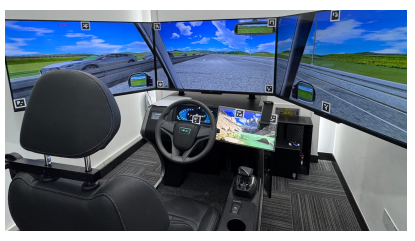
\includegraphics[width=0.6\textwidth]{fig1.png}
    \caption{The driving simulator setup used in the experiment.}
    \label{fig:simulator}
\end{figure}

\subsection{Scenario Design and Driving Tasks}

The experimental driving environment consisted of an 8-kilometer-long, three-lane highway with three exit ramps distributed along its length. The highway had a posted speed limit of 80 km/h. To replicate realistic highway traffic conditions with moderate congestion levels, we configured the simulation to include ambient traffic at a density of 20 vehicles per kilometer. Vehicles maintained an average bumper-to-bumper spacing of 20 meters and traveled at an average speed of approximately 60 km/h. This moderate congestion level was specifically chosen because it creates challenging lane-change conditions where gaps between vehicles are relatively small, making explicit communication potentially more valuable.

Participants received instructions to maintain their position in the middle lane whenever possible, follow the lead vehicle at a safe distance, and drive as they would in real-world highway conditions. The critical experimental manipulation occurred during lane-change events. When the participant's vehicle reached a distance of 200 meters from an exit ramp, a target vehicle (the cutting-in vehicle) positioned 50 meters behind in the leftmost lane was triggered to accelerate. This vehicle accelerated from its initial speed of 60 km/h at a rate of 6 m/s² until reaching a position approximately 15 meters ahead of the participant's vehicle. This acceleration phase lasted approximately 4 seconds, after which the cutting-in vehicle initiated its lane-change maneuver.

The cutting-in vehicle executed two consecutive lane changes: first from the leftmost lane to the middle lane (directly in front of the participant), and then from the middle lane to the rightmost lane before exiting via the on-ramp. This two-stage maneuver created a realistic and challenging scenario requiring participants to make real-time decisions about whether to yield to the cutting-in vehicle or maintain their speed and position.

Each experimental drive included four such lane-change events, spaced at intervals along the highway to avoid habituation effects while maintaining ecological validity. The spacing between events was sufficient to allow participants to return to normal driving before encountering the next event.

\begin{figure}[htbp]
    \centering
    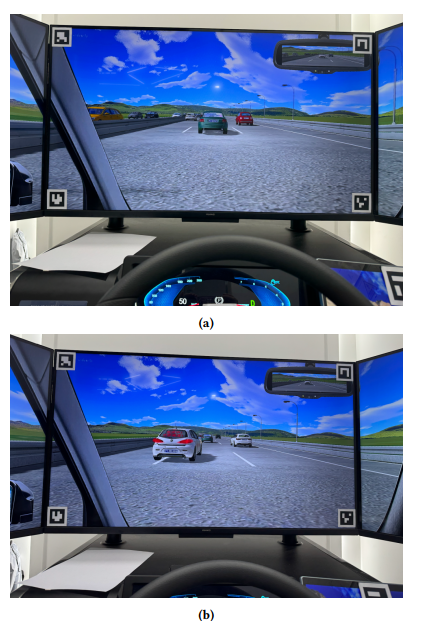
\includegraphics[width=0.75\textwidth]{fig2.png}
    \caption{Driving scenarios: (a) Normal driving scenario showing the three-lane highway; (b) Lane-changing scenario with the cutting-in vehicle.}
    \label{fig:scenarios}
\end{figure}

\begin{figure}[htbp]
    \centering
    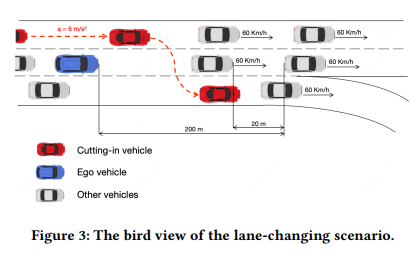
\includegraphics[width=0.65\textwidth]{fig3.png}
    \caption{Bird's-eye view schematic illustrating the lane-changing scenario geometry and vehicle positions.}
    \label{fig:birdview}
\end{figure}

\subsection{eHMI Designs}

We designed three distinct text-based eHMI conditions plus a baseline control condition without eHMI. All eHMI messages were displayed in red text on both the rear window and side panels of the cutting-in vehicle to ensure maximum visibility from the participant's viewing position. The red color was selected based on previous eHMI research \cite{dey2020taming} showing that high-salience colors improve message detection and processing, particularly when drivers are not expecting such displays.

The four experimental conditions were:

\textbf{Baseline (No eHMI):} The cutting-in vehicle used only standard automotive signals (turn indicators and brake lights) without any text-based eHMI communication.

\textbf{Command eHMI:} Displayed the message "Changing lanes, slow down immediately." This condition was designed to test direct, imperative communication based on research showing that clear commands can facilitate rapid responses in emergency situations \cite{merat2012highly, parasuraman1997humans}.

\textbf{Polite eHMI:} Displayed the message "Changing lanes, please yield to me." This condition was grounded in Politeness Theory \cite{brown1987politeness}, testing whether respectful requests increase compliance through positive social framing.

\textbf{Explanatory eHMI:} Displayed the message "About to exit ramp, preparing for lane change." This condition provided contextual justification for the lane-change maneuver, based on social psychology research showing that explanations enhance cooperation \cite{burger2004coincidence}.

The eHMI messages appeared as soon as the cutting-in vehicle began its acceleration phase and remained visible throughout the entire two-stage lane-change maneuver until the vehicle completed its exit from the highway. This timing ensured that participants had sufficient opportunity to perceive and process the communicated information before needing to make their yielding decision.

\begin{figure}[htbp]
    \centering
    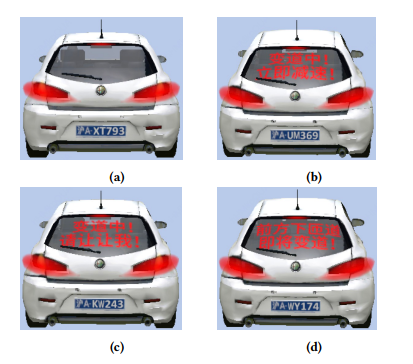
\includegraphics[width=0.85\textwidth]{fig4.png}
    \caption{The four eHMI conditions: (a) Baseline with no eHMI; (b) Command eHMI stating "Changing lanes, slow down immediately"; (c) Polite eHMI stating "Changing lanes, please yield to me"; (d) Explanatory eHMI stating "About to exit ramp, preparing for lane change".}
    \label{fig:ehmi_designs}
\end{figure}

\subsection{Experimental Design}

The study employed a within-subjects experimental design with eHMI type as the independent variable. This design was chosen to maximize statistical power while controlling for individual differences in driving style and decision-making tendencies. Each participant experienced all four eHMI conditions (baseline, command, polite, and explanatory) across four separate driving sessions.

To minimize order effects and learning biases, we counterbalanced the presentation order of conditions using a Latin square design. This resulted in four distinct condition orders, with each order assigned to exactly eight participants (four males and four females). Additionally, each driving session contained four lane-change events, allowing us to collect multiple observations per condition while maintaining scenario realism. This design yielded a total of 512 lane-change events across all participants (32 participants × 4 drives × 4 events per drive).

\subsection{Procedure}

Upon arrival at the laboratory, participants were greeted by the experimenter and provided with an overview of the study procedures. After reviewing and signing the informed consent form, participants received comprehensive training on simulator operation. This training phase included familiarization with the vehicle controls, acceleration and braking characteristics, and the visual display system.

Following the training, participants completed a practice drive lasting approximately 5 minutes. This demo drive served to acclimate participants to the simulator's handling characteristics and reduce the potential for simulator adaptation effects during the experimental trials. Participants were instructed to drive along the highway as they would in real-world conditions, maintaining position in the middle lane when possible, following the lead vehicle at a safe distance, and responding naturally to surrounding traffic.

Critically, participants were not informed about the eHMI system or its purpose during the briefing or training phases. This decision was intentional to avoid priming effects \cite{nichols2008good, rosenthal2009artifacts, orne2002social} and allow participants to interpret the eHMI messages based on their spontaneous perceptions and prior driving experience. This approach enhanced the ecological validity of the study by simulating how drivers might naturally respond to novel vehicle communication systems encountered without prior explanation.

After completing the practice drive, participants began the four experimental drives. Each drive lasted approximately 10 minutes and contained four lane-change events distributed along the highway route. Brief rest periods were provided between drives to minimize fatigue effects. Following completion of all experimental drives, participants completed the System Usability Scale (SUS) questionnaire \cite{brooke1996sus} to evaluate their subjective perceptions of each eHMI type and the baseline interaction condition. The SUS is a validated 10-item scale widely used in usability research, providing scores ranging from 0 to 100.

Finally, participants were asked open-ended questions about their experience with the eHMI displays, including what they noticed, how the messages influenced their driving decisions, and any suggestions for improving the interface designs. This qualitative feedback provided valuable insights into participants' conscious awareness and interpretation of the communication strategies. The entire experimental session lasted approximately 90 minutes per participant.

\subsection{Dependent Variables and Statistical Analysis}

We employed both objective behavioral measures and subjective evaluations to comprehensively assess eHMI effectiveness. The primary objective measures were:

\textbf{Yield Rate:} Defined as the proportion of lane-change events in which the participant yielded to the cutting-in vehicle by reducing speed to allow the vehicle to complete its maneuver safely. This binary outcome (yield/no yield) was coded for each of the 512 observed events based on analysis of the recorded vehicle trajectory and speed data.

\textbf{Minimum Time-to-Collision (minTTC):} Calculated as the smallest time interval until a potential collision would occur between the participant's vehicle and the cutting-in vehicle, assuming both vehicles maintained constant speeds and trajectories. TTC was computed continuously throughout each lane-change event using the formula from \cite{hwang2022autonomous}, and the minimum value was extracted as representing the moment of highest collision risk. Lower minTTC values indicate more dangerous situations with smaller safety margins.

The subjective measure was:

\textbf{System Usability Scale (SUS) Score:} Participants rated each eHMI condition using the standardized 10-item SUS questionnaire \cite{brooke1996sus}. Responses were converted to a composite score ranging from 0 (poorest usability) to 100 (best usability) following standard SUS scoring procedures.

All statistical analyses were conducted using SAS On Demand for Academics. For the analysis of yield rates (a binary outcome), we employed a Poisson regression model with generalized estimating equations (GEE) \cite{liang1986longitudinal} to account for repeated measurements from the same participants. For the continuous outcomes (minTTC and SUS scores), we used Linear Mixed Models (LMM) with random intercepts for participants.

In all models, we included eHMI type (four levels: baseline, command, polite, explanatory) and participant gender (two levels: male, female) as fixed effects, along with their two-way interaction term. This allowed us to test whether gender moderated the effects of eHMI type on driver responses, given previous research suggesting gender differences in technology acceptance \cite{venkatesh2000why}. When overall effects reached statistical significance (α = 0.05), we conducted post-hoc pairwise comparisons. For yield rate comparisons, we used Wald tests. For minTTC and SUS score comparisons, we applied Tukey's Honestly Significant Difference (HSD) procedure to control for family-wise error rate across multiple comparisons.

\section{Findings and Results}

\subsection{Yield Rate}

The analysis of yielding behavior revealed a highly significant main effect of eHMI type on yield rates (χ²(3) = 45.65, p < .001), confirming that the presence and type of external communication substantially influenced participants' decisions to yield to cutting-in vehicles. Participant gender did not demonstrate a significant main effect on yielding behavior (p = .2), nor was there a significant interaction between eHMI type and gender (p > .05), indicating that the eHMI effects were consistent across male and female participants.

Figure \ref{fig:yield_rates} illustrates the yield rate distributions across the four experimental conditions. As shown in the figure, darker colors represent higher numbers of yielding instances out of the 32 possible trials per condition. The baseline condition without eHMI resulted in the lowest yield rate, with participants yielding in only a minority of encounters. In contrast, all three eHMI conditions produced substantially higher yield rates, with the polite eHMI condition demonstrating the highest compliance.

\begin{figure}[htbp]
    \centering
    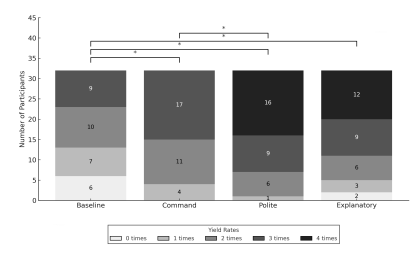
\includegraphics[width=0.6\textwidth]{fig5.png}
    \caption{Yield rates across different eHMI conditions. Darker colors indicate higher numbers of yielding instances. Asterisks (*) denote statistically significant pairwise differences (p < .05).}
    \label{fig:yield_rates}
\end{figure}

Post-hoc pairwise comparisons (Table \ref{tab:comparison_objective}) revealed that each eHMI condition significantly increased yield rates compared to the baseline. The polite eHMI produced the largest improvement (Δ = -0.655, 95\% CI: -0.984 to -0.327, p < .001), followed by the explanatory eHMI (Δ = -0.511, 95\% CI: -0.848 to -0.173, p = .003) and the command eHMI (Δ = -0.355, 95\% CI: -0.703 to -0.007, p = .046). Furthermore, direct comparison between eHMI types revealed that the polite eHMI significantly outperformed the command eHMI (Δ = 0.301, 95\% CI: 0.006 to 0.595, p = .046), while the difference between polite and explanatory eHMIs did not reach statistical significance (p = .315).

\subsection{Minimum Time-to-Collision}

The analysis of safety margins, as measured by minimum time-to-collision, also demonstrated a highly significant main effect of eHMI type (F(3,93) = 50.5, p < .001). Consistent with the yield rate findings, participant gender showed no significant main effect (p = .2) and did not interact with eHMI type.

Figure \ref{fig:minttc} presents boxplots showing the distribution of minTTC values across conditions. The boxplots display the minimum, first quartile, median, third quartile, and maximum values, with the 'x' symbol indicating the group mean. As evident from the figure, the baseline condition produced the smallest minTTC values (M = 2.38 seconds), indicating the highest collision risk. All three eHMI conditions substantially increased minTTC, with the polite eHMI yielding the largest safety margins (M ≈ 5.2 seconds).

\begin{figure}[htbp]
    \centering
    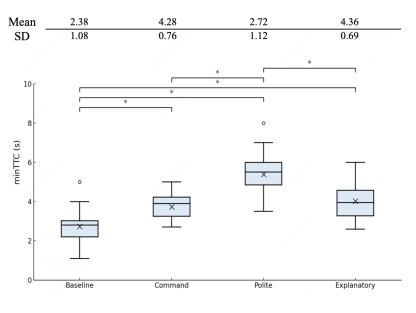
\includegraphics[width=0.6\textwidth]{fig6.png}
    \caption{Minimum Time-to-Collision (minTTC) across different eHMI conditions. Boxplots show the distribution of safety margins, with 'x' indicating group means. Higher values indicate greater safety margins.}
    \label{fig:minttc}
\end{figure}

Pairwise comparisons (Table \ref{tab:comparison_objective}) confirmed that all eHMI types significantly improved safety compared to baseline: command eHMI increased minTTC by 1.003 seconds (95\% CI: 0.580 to 1.426, p < .001), explanatory eHMI by 1.294 seconds (95\% CI: 0.871 to 1.716, p < .001), and polite eHMI by 2.806 seconds (95\% CI: 2.384 to 3.229, p < .001). Among the eHMI types, the polite interface produced significantly larger safety margins than both the command (Δ = 1.803 seconds, 95\% CI: 1.379 to 2.226, p < .001) and explanatory (Δ = 1.512 seconds, 95\% CI: 0.943 to 2.091, p < .001) interfaces. The command and explanatory eHMIs did not differ significantly from each other in terms of minTTC (p = .358).

\begin{table}[h]
\centering
\caption{Pairwise comparisons across eHMI conditions on Yield Rates and minTTC.}
\label{tab:comparison_objective}
\begin{tabular}{lccccc}
\toprule
 & \multicolumn{2}{c}{\textbf{Yield Rates}} & & \multicolumn{2}{c}{\textbf{minTTC}} \\
\cmidrule{2-3} \cmidrule{5-6}
\textbf{Comparison} & \textbf{Δ (95\% CI)} & \textbf{p} & & \textbf{Δ (95\% CI)} & \textbf{p} \\
\midrule
Baseline vs Command & -0.355 (-0.703, -0.007) & .046 & & -1.003 (-1.426, -0.580) & <.001 \\
Baseline vs Polite & -0.655 (-0.984, -0.327) & <.001 & & -2.806 (-3.229, -2.384) & <.001 \\
Baseline vs Explanatory & -0.511 (-0.848, -0.173) & .003 & & -1.294 (-1.716, -0.871) & <.001 \\
Polite vs Command & 0.301 (0.006, 0.595) & .046 & & 1.803 (1.379, 2.226) & <.001 \\
Polite vs Explanatory & 0.145 (-0.138, 0.427) & .315 & & 1.512 (0.943, 2.091) & <.001 \\
Command vs Explanatory & -0.156 (-0.461, 0.148) & .315 & & -0.291 (-0.693, 0.115) & .358 \\
\bottomrule
\end{tabular}
\end{table}

\subsection{Subjective Usability Ratings}

Participants' subjective evaluations of the eHMI systems, as measured by System Usability Scale scores, revealed significant differences across conditions (F(3,124) = 36.47, p < .001). No other main effects or interactions reached statistical significance.

Figure \ref{fig:sus} displays the distribution of SUS scores across the four conditions. The polite eHMI received the highest usability ratings (M ≈ 77), which falls in the "good" to "excellent" usability range according to standard SUS interpretation guidelines. The explanatory eHMI received the second-highest ratings (M ≈ 71), still in the "good" range. The command eHMI received notably lower ratings (M ≈ 52), placing it in the "marginal" usability category. The baseline condition, relying solely on traditional signals, received the lowest scores (M ≈ 39), indicating "poor" perceived usability.

\begin{figure}[htbp]
    \centering
    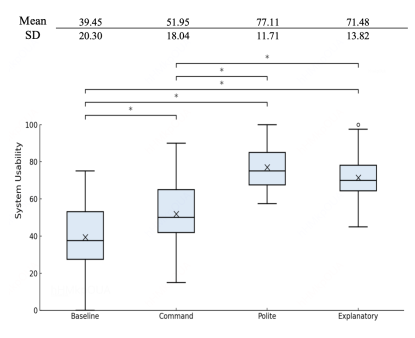
\includegraphics[width=0.6\textwidth]{fig7.png}
    \caption{System Usability Scale (SUS) scores across different eHMI conditions. Higher scores indicate better perceived usability.}
    \label{fig:sus}
\end{figure}

Post-hoc pairwise comparisons (Table \ref{tab:comparison_sus}) revealed that all three eHMI conditions received significantly higher usability ratings than the baseline: command eHMI showed an improvement of 12.51 points (95\% CI: 1.87 to 23.13, p = .014), explanatory eHMI improved by 32.03 points (95\% CI: 21.41 to 42.66, p < .001), and polite eHMI showed the largest improvement of 37.66 points (95\% CI: 27.03 to 48.29, p < .001).

Comparisons among the eHMI types themselves revealed additional nuances. The polite eHMI was rated significantly more usable than the command eHMI (Δ = 25.16, 95\% CI: 14.53 to 35.79, p < .001), but the difference between polite and explanatory eHMIs was not statistically significant (p = .515). The explanatory eHMI also received significantly higher ratings than the command eHMI (Δ = -19.53, 95\% CI: -30.16 to -8.90, p < .001).

\begin{table}[h]
\centering
\caption{Pairwise comparisons across eHMI conditions on SUS scores.}
\label{tab:comparison_sus}
\begin{tabular}{lcc}
\toprule
\textbf{Comparison} & \textbf{Δ (95\% CI)} & \textbf{p-value} \\
\midrule
Baseline vs Command & -12.51 (-23.13, -1.87) & .014 \\
Baseline vs Polite & -37.66 (-48.29, -27.03) & <.001 \\
Baseline vs Explanatory & -32.03 (-42.66, -21.41) & <.001 \\
Polite vs Command & 25.16 (14.53, 35.79) & <.001 \\
Polite vs Explanatory & 5.63 (-5.01, 16.25) & .515 \\
Command vs Explanatory & -19.53 (-30.16, -8.90) & <.001 \\
\bottomrule
\end{tabular}
\end{table}

These subjective findings closely paralleled the objective behavioral results, suggesting that participants' conscious perceptions of interface quality aligned well with their actual behavioral responses. The consistency between objective and subjective measures strengthens confidence in the validity of our findings.

\section{Discussion}

The results of this study provide compelling evidence for the efficacy of external Human-Machine Interfaces in vehicle-to-vehicle interactions during lane-changing scenarios. Our findings address both research questions and support both hypotheses, while also revealing important nuances regarding the role of communicative tone in eHMI design.

\subsection{Effects of eHMI Presence}

Addressing RQ1, we found clear support for H1: the presence of any form of eHMI significantly improved both yielding rates and safety margins compared to the baseline condition relying solely on traditional turn signals. This confirms that the ambiguity inherent in conventional lane-changing scenarios where drivers must infer intentions from implicit cues like vehicle position and blinkers represents a substantial safety liability. By providing explicit textual communication of lane-change intentions, eHMIs effectively reduced this uncertainty and facilitated more cooperative interactions between vehicles.

These findings extend previous research on eHMI effectiveness from the AV-pedestrian domain \cite{habibovic2018communicating, colley2021investigating} into the more dynamic and complex realm of V2V interactions. The fact that explicit communication improved outcomes even when both vehicles were human-driven (rather than involving AVs) suggests that the benefits of eHMIs are not limited to bridging the human-machine gap but rather address a more fundamental challenge in traffic interaction: the difficulty of accurately communicating intentions in time-critical scenarios.

The magnitude of the safety improvement is noteworthy. The polite eHMI increased minimum time-to-collision by nearly 3 seconds compared to baseline a difference that could be critical in preventing collisions. Even the less effective command eHMI still provided a 1-second safety buffer improvement. These results demonstrate that explicit intention communication can yield substantial real-world safety benefits.

\subsection{Effects of eHMI Tone}

Addressing RQ2, our results strongly support H2: different communicative tones produced significantly different behavioral and subjective outcomes. The polite eHMI consistently outperformed both the command and explanatory variants across all dependent measures, yielding the highest compliance rates, largest safety margins, and best usability ratings.

This pattern of results aligns closely with Politeness Theory \cite{brown1987politeness}. The polite phrasing ("please yield to me") appears to have activated social norms of cooperation and reciprocity, making drivers more willing to accommodate the lane-change request. In contrast, the commanding tone ("slow down immediately"), despite its clarity and directness, may have triggered psychological reactance a negative emotional response to perceived threats to behavioral freedom. Even though the command clearly communicated the desired action, its authoritarian framing reduced rather than enhanced compliance.

The explanatory eHMI presented an interesting middle ground. While it did not match the polite interface in behavioral outcomes, it received comparably high usability ratings. This suggests that providing contextual justification ("about to exit ramp") helped participants understand and accept the lane-change maneuver, even if the phrasing itself was less compelling than the polite request. This finding aligns with social psychology research on the power of explanations \cite{burger2004coincidence} and suggests that transparency about driving motivations can enhance acceptance of eHMI communication.

Interestingly, the command and explanatory eHMIs produced equivalent safety outcomes (minTTC), despite significant differences in perceived usability. This dissociation suggests that while both interfaces successfully communicated the lane-change intention, the social framing of that communication substantially affected how drivers consciously experienced and evaluated the interaction. Such findings have important implications for long-term acceptance and adoption of eHMI systems: interfaces that feel uncomfortable or aggressive may face user resistance even when technically effective.

\subsection{Implications for eHMI Design}

Our findings carry several important implications for the design of external communication systems for both human-driven and autonomous vehicles. First, the results demonstrate that explicit communication of driving intentions through eHMIs can significantly enhance both safety and efficiency in dynamic V2V scenarios. As vehicles become increasingly connected and automated, incorporating such explicit communication capabilities could yield substantial traffic safety benefits.

Second, and perhaps more importantly, our results highlight that the content of communication is not the only consideration how information is framed and conveyed matters enormously. Designers must consider not only what information to communicate but also how to phrase that information in ways that align with social norms and expectations. Cooperative, respectful communication appears more effective than authoritative commands, at least in non-emergency scenarios.

Third, the success of the explanatory eHMI suggests value in providing contextual information alongside intention statements. While "I am changing lanes" communicates what is happening, "I am exiting" explains why, potentially increasing other drivers' understanding and willingness to cooperate. Future eHMI systems might benefit from combining polite requests with brief contextual explanations.

Fourth, the consistency between objective behavioral measures and subjective usability ratings suggests that drivers are reasonably aware of how different communication styles affect their driving decisions. This conscious awareness could facilitate user acceptance of eHMI technologies, particularly if systems employ communication strategies that feel natural and respectful.

\subsection{Limitations and Future Directions}

Several limitations of this study should be acknowledged and addressed in future research. First, the use of a driving simulator, while providing excellent experimental control and safety, necessarily limits ecological validity. Real-world driving involves genuine physical risk, varied weather and lighting conditions, and more complex traffic scenarios than could be simulated. Field studies or naturalistic driving studies would provide valuable validation of these findings under actual road conditions.

Second, our participant sample, while gender-balanced, consisted primarily of young drivers (mean age 28) with relatively limited driving experience (mean 4.75 years). Older drivers with decades of experience might respond differently to novel eHMI systems. Similarly, cultural factors could play an important role in how drivers interpret different communicative tones \cite{ehrhardt2024comparing, lundgren2017new}. Cross-cultural validation studies would be valuable for understanding the generalizability of our findings.

Third, participants were not informed whether cutting-in vehicles were autonomous or human-driven. While this design choice avoided confounding eHMI effects with attitudes toward automation, it limits our understanding of how vehicle type might moderate eHMI effectiveness. Previous research suggests humans may interact differently with AVs versus human-driven vehicles \cite{huang2022sharing, stanton2020turing}, and future studies should explicitly manipulate and measure this factor.

Fourth, we employed text-based eHMIs to maximize interpretability and isolate the effects of communicative tone. However, text displays require visual attention and reading time, which could be problematic in some traffic situations. Future research should explore multimodal eHMI designs combining text with icons, light patterns, or dynamic visual displays that could convey similar information more rapidly or intuitively. Recent work has begun exploring such multimodal approaches \cite{liu2025where}, and extending our tone-based findings to these richer display formats would be valuable.

Fifth, our study examined lane-changing scenarios specifically. While these are common and important maneuvers, V2V communication could potentially benefit other scenarios such as merging, yielding at intersections, or navigating parking situations. The relative effectiveness of different communicative tones might vary across these contexts, particularly in emergency situations where direct commands might prove more effective than polite requests.

Sixth, while the System Usability Scale provided valuable subjective data, it was originally designed for evaluating interactive systems used directly by the person completing the scale. In our study, participants were evaluating communication they received from external vehicles, which represents a somewhat different use case. Future research might benefit from developing or adapting subjective measures specifically designed for evaluating external vehicle communication.

Finally, our study did not account for individual differences in driving style, personality, or susceptibility to different forms of social influence. Previous research has shown that such individual differences can moderate responses to framing and persuasive communication \cite{anderson2010framing}. Understanding which drivers respond most positively to which communication styles could enable personalized or adaptive eHMI systems that tailor their communication to individual preferences or situational demands.

\subsection{Broader Context and Future Applications}

Despite these limitations, this study represents an important first step in understanding how eHMIs can facilitate safer and more efficient V2V interactions among human-driven vehicles. As the automotive industry continues its gradual transition toward vehicle automation, mixed-traffic environments containing both human-driven and autonomous vehicles will persist for decades. Effective V2V communication systems that work well for both human and automated vehicles will be essential during this transition period.

Moreover, even in a fully autonomous future, human passengers and other road users will still need to understand vehicle intentions. The principles identified in this study regarding respectful, clear, and contextual communication are likely to remain relevant regardless of who or what is controlling the vehicle. The finding that polite, cooperative communication outperforms authoritative commands suggests broader lessons about human-machine interaction that extend beyond the specific domain of vehicle communication.

Looking forward, several exciting research directions emerge from this work. First, investigating how eHMI communication might be dynamically adapted based on traffic density, urgency level, or individual driver characteristics could yield more sophisticated and effective systems. Second, exploring how eHMIs might facilitate more complex negotiations in multi-vehicle scenarios such as four-way stop intersections or roundabouts represents an important extension. Third, examining the long-term effects of widespread eHMI adoption on driving behavior and traffic culture could reveal emergent phenomena not visible in short-term studies.

\section{Conclusion}

This study investigated the effectiveness of external Human-Machine Interfaces for communicating lane-change intentions in vehicle-to-vehicle interactions among human-driven vehicles. Through a controlled driving simulator experiment with 32 participants, we examined how three different eHMI tones (command, polite, and explanatory) influenced drivers' yielding behavior, safety margins, and subjective usability perceptions compared to a baseline condition with only traditional turn signals.

Our results demonstrate clear and substantial benefits of explicit intention communication. All three eHMI types significantly increased yielding rates and minimum time-to-collision compared to the baseline, confirming that reducing ambiguity through explicit communication enhances both cooperation and safety in lane-changing scenarios. Critically, we found that communicative tone significantly moderated these effects, with polite phrasing consistently producing the best outcomes across both objective behavioral measures and subjective usability ratings. This finding underscores that effective eHMI design requires careful consideration not only of what information to convey but how to convey it in ways that align with social norms and expectations.

These findings contribute to the growing body of research on external vehicle communication systems by extending previous work from AV-pedestrian interactions into the more dynamic domain of V2V interactions and by providing the first systematic investigation of how communicative tone affects driver responses in lane-changing scenarios. As vehicles become increasingly connected and automated, the principles identified in this study regarding respectful, clear, and contextual communication can inform the design of eHMI systems that facilitate safer, more efficient, and more socially acceptable traffic interactions.

While future research must address the limitations of this initial investigation particularly through real-world validation, broader participant samples, and exploration of multimodal interface designs this study establishes a foundation for understanding how explicit external communication can enhance V2V interactions. By demonstrating that polite, cooperative communication outperforms authoritative commands, we provide actionable guidance for designers and engineers developing the next generation of vehicle communication systems.

\bibliographystyle{ACM-Reference-Format}
\bibliography{references}

\end{document}